%%%%%%%%%%%%%%%%%%%%%%%%%%%%%%%%%%%%%%%%%
% Thin Sectioned Essay
% LaTeX Template
% Version 1.0 (3/8/13)
%
% This template has been downloaded from:
% http://www.LaTeXTemplates.com
%
% Original Author:
% Nicolas Diaz (nsdiaz@uc.cl) with extensive modifications by:
% Vel (vel@latextemplates.com)
%
% License:
% CC BY-NC-SA 3.0 (http://creativecommons.org/licenses/by-nc-sa/3.0/)
%
%%%%%%%%%%%%%%%%%%%%%%%%%%%%%%%%%%%%%%%%%

%----------------------------------------------------------------------------------------
%	PACKAGES AND OTHER DOCUMENT CONFIGURATIONS
%----------------------------------------------------------------------------------------

\documentclass[a4paper, 12pt]{article} % Font size (can be 10pt, 11pt or 12pt) and paper size (remove a4paper for US letter paper)

\usepackage[protrusion=true,expansion=true]{microtype} % Better typography
\usepackage{graphicx} % Required for including pictures
\usepackage[utf8]{inputenc}
\usepackage[margin=1.0in]{geometry}
\usepackage{url}
\usepackage{fancyhdr}
\usepackage{amsmath}
\usepackage{setspace}
\usepackage{enumitem}
\setlength\parindent{0pt} % Removes all indentation from paragraphs

\usepackage[T1]{fontenc} % Required for accented characters
\usepackage{times} % Use the Palatino font

\usepackage{listings}
\usepackage{color}
\lstset{mathescape}

\definecolor{dkgreen}{rgb}{0,0.6,0}
\definecolor{gray}{rgb}{0.5,0.5,0.5}
\definecolor{mauve}{rgb}{0.58,0,0.82}

\lstset{frame=tb,
   language=c++,
   aboveskip=3mm,
   belowskip=3mm,
   showstringspaces=false,
   columns=flexible,
   basicstyle={\small\ttfamily},
   numbers=none,
   numberstyle=\tiny\color{gray},
   keywordstyle=\color{blue},
   commentstyle=\color{dkgreen},
   stringstyle=\color{mauve},
   breaklines=true,
   breakatwhitespace=true
   tabsize=3
}
\linespread{1.25} % Change line spacing here, Palatino benefits from a slight increase by default

\makeatletter
\renewcommand{\@listI}{\itemsep=0pt} % Reduce the space between items in the itemize and enumerate environments and the bibliography

\renewcommand\abstractname{Résumé}
\renewcommand\refname{Références}
\renewcommand\contentsname{Table des matières}
\renewcommand{\maketitle}{ % Customize the title - do not edit title and author name here, see the TITLE block below
\begin{center} % Right align

\vspace*{25pt} % Some vertical space between the title and author name
{\LARGE\@title} % Increase the font size of the title

\vspace{125pt} % Some vertical space between the title and author name

{\large\@author} % Author name

\vspace{125pt} % Some vertical space between the author block and abstract
Dans le cadre du cours
\\INF8702 - Infographie avancée
\vspace{125pt} % Some vertical space between the author block and abstract
\\\@date % Date
\vspace{125pt} % Some vertical space between the author block and abstract

\end{center}
}

%----------------------------------------------------------------------------------------
%	TITLE
%----------------------------------------------------------------------------------------

\title{Rapport final: Génération de vague à l'aide de particule} 

\author{\textsc{Guillaume Arruda 1635805\\Raphael Lapierre 1644671} % Author
\vspace{10pt}
\\{\textit{École polytechnique de Montréal}}} % Institution

\date{8 Décembre 2015} % Date

%----------------------------------------------------------------------------------------

\begin{document}

\thispagestyle{empty}
\clearpage\maketitle % Print the title section
\pagebreak[4]
\tableofcontents
\pagebreak[4]
%----------------------------------------------------------------------------------------
%	En tête et pieds de page 
%----------------------------------------------------------------------------------------

\setlength{\headheight}{15.0pt}
\pagestyle{fancy}
\fancyhead[L]{INF8702}
\fancyhead[C]{}
\fancyhead[R]{Rapport final}
\fancyfoot[C]{\textbf{page \thepage}}

%----------------------------------------------------------------------------------------
%	ESSAY BODY
%----------------------------------------------------------------------------------------
\section{Introduction}
    \paragraph{}
    Dans le cadre du cours d'infographie avancée, un projet final au choix de l'étudiant 
    devait être réalisé. Lors des dernières semaines, ce dernier a donc été choisi et implémenté.
    Le but du présent travail est donc de présenter, sous forme de rapport, le fruit de notre
    travail des dernières semaines.

\subsection{Problématique}
    \paragraph{}
    De manière très générale, nous désirions, pour notre travail de session, implémenter 
    le rendu d'une surface d'eau de façon réaliste et de simuler des vagues sur celle-ci.
    Pour réussir à atteindre ce but, plusieurs éléments se devaient d'être présents pour notre
    simulation. Niveau lumière, il est impératif de pouvoir compter sur des effets de réflexion
    et de réfraction. En effet, une surface d'eau laissera pénétrer une partie de la lumière
    ce qui causera de la réfraction et une partie de la lumière sera réfléchie ce qui donnera
    la réflexion.

    \paragraph{}
    L'autre partie importante est d'avoir une simulation de vagues sur l'eau qui est assez
    proche de la réalité physique de la situation pour que l'illusion soit complète pour 
    l'humain. Pour se faire, un système de particule se déplaçant en suivant une propagation
    respectant l'équation d'onde a été utilisé. La théorie derrière notre simulation sera 
    présentée plus en détail dans la section
    suivante du rapport.

\section{Théorie}
    \paragraph{}
    Il est naturel dans cette section de séparer la théorie en trois parties.
    On parle ici de la théorie des \textit{wave-particle}, de la réflexion et finalement,
    de la réfraction.

    \subsection{Wave-Particle}
        \paragraph{}
    	Dans ce travail, la simulation des vagues a été réalisée à l'aide d'une technique
	qui se nomme \textit{Wave-Particle}. Cette dernière a été mise au point par Cem
	Yuskel lors de son doctorat à l'université de Bogazici en Turquie.\cite{Yuskel}
	Il s'agit d'une technique qui peut sembler assez complexe à première vue mais elle
	s'avère assez simple une fois que l'on comprend bien les différentes parties.

        \paragraph{}
	L'idée générale est de simuler des particules qui se déplacent sur la surface de l'eau.
	À chacune des ces particules est confié un rayon d'influence ainsi qu'une amplitude.
	La hauteur de l'eau en chaque point où une particule est située est donc ajustée 
	suivant une fonction qui sera présentée plus tard, pour arriver à un front d'onde
	qui semblera continue dû au grand nombre de particules et leurs rayons d'influence.
	Voici donc sous forme de listes toutes les caractéristiques que nous avons attribuées
	à nos particules.

	\begin{itemize}
	    \item Position initial
	    \item Vitesse
	    \item Direction
	    \item Temps de vie total
	    \item Rayon d'influence
	    \item Amplitude
	    \item Angle de dispersion
	\end{itemize}

	\paragraph{}
	Avec la position initial, le temps de vie, la direction et la vitesse, il est possible de 
	déterminer à tout instant la position d'une de nos particules. On peut voir un exemple des particules
	isolés pour pouvoir mieux observer leurs différentes caractéristiques à la figure \ref{NoSubdivide}.
	Pour que le front d'onde simulé ait l'air de se propager bel et bien comme une vague
	sur l'eau, les particules doivent se déplacer suivant une équation mathématique respectant
	l'équation d'onde (équation différentielle) suivante.

	\begin{figure}
		\centering
		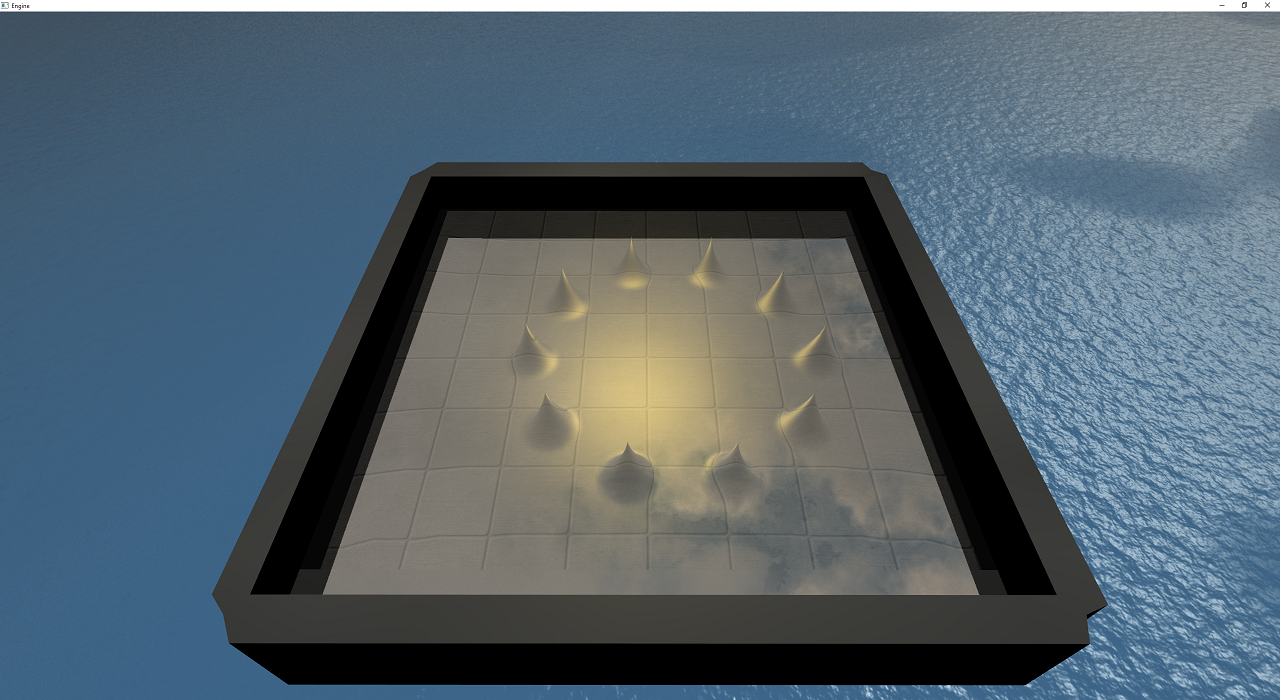
\includegraphics[width=0.9\textwidth]{./PhotoRapport/NoSubdivide.png}
		\caption{Sans subdivision}
		\label{NoSubdivide}
	\end{figure}

	\begin{equation}
	    \frac{\partial^{2}u}{\partial t^{2}} = c^{2} \frac {\partial^{2}u} {\partial x^{2}}
	\end{equation}

	\paragraph{}
	On comprend donc maintenant pourquoi le temps de vie total de chaque particule est conservée.
	Cette équation dépend, pour déterminer la position d'une particule, du temps et aussi de sa position.
	Il y a donc deux déplacements pour nos particules à prendre en compte lorsqu'on cherche une solution à
	l'équation d'onde. Le premier est le déplacement horizontale de nos particules, celui dans le plan.
	Pour respecter l'équation d'onde une vitesse constante de déplacement est le requis, un peu à la façon
	où la lumière se déplace toujours à $c$ peu importe la situation. C'est donc de cette façon que nos particules
	se déplaçait. En ce qui a trait à la hauteur des particules, une autre équation, déterminée par Cem Yuskel,
	a été utilisée. Celle-ci respecte, encore une fois, l'équation d'onde et donne une forme et un résultat satisfaisant
	aux vagues. La voici :

	\begin{equation}
	    D_{i}(x, t) = \frac{a_{i}}{2} \left( \cos\left( \frac{\pi |x - x_{i}(t)|}{r_{i}}\right) + 1\right)
	    \Pi \left( \frac{|x - x_{i}(t)|} {2 r_{i}}\right)
	\end{equation}

	\paragraph{}
	Dans cette équation, l'indice $i$ dénote la \textit{ième} particule, $a_{i}$ l'amplitude, $x_{i}$ la position de la particule,
	$x$ le point de la surface ou la hauteur est affectée,
	$r_{i}$ le rayon de la particule et $\Pi$ la fonction rectangle. Finalement, en combinant le déplacement horizontal et vertical des particules sur 
	les points de la surface de l'eau faisant partie de leurs rayons d'influence, il est possible de simuler une vague sur l'eau.
	Par contre, il manque encore quelques détails pour permettre à nos vagues d'être plus réalistes.

	\subsubsection{Ajustement horizontal}
	Une limitation de la méthode utilisé pour simuler les particules se trouve dans le fait que notre simulation se passe 
	entièrement en deux dimensions. Bien évidemment, l'eau est un fluide qui, lorsqu'elle fait des vagues, s'étend dans trois dimensions.
	Pour simuler le déplacement horizontal du dessus d'une vague sur le point de casser, un dernier déplacement doit être appliqué
	par les particules.

	\subsubsection{Subdivision des particules}
	\subsubsection{Réflection des particules}


\section{Implémentation}
\subsection{Introduction au moteur graphique}
	\paragraph{}
	Le moteur graphique a été écrit pour nous familiariser avec OpenGL 4.4. Il utilise les librairies suivantes:
	\begin{description}
		\item[Assimp] pour le chargement des modèles 3D
		\item[DevIL] pour le chargement des textures
		\item[glfw3] pour la création des fenêtre
		\item[tinyxml2] pour la lecture des fichiers xml
		\item[glew] pour faciliter l'utilisation de OpenGL
		\item[OpenMP] pour faciliter la mise en parallèle de l'application
	\end{description}
	
	\paragraph{}
	Son fonctionnement est simple. Il utilise un arbre de rendu qui appelle la fonction "Update" qui met à jour les noeuds de l'arbre.
	L'arbre de rendu appelle ensuite les fonctions "Render*" qui affiche les noeuds à l'écran. L'arbre de rendu est créé à l'aide du
	fichier "MainRenderTree.xml" et l'environnement qui décrit les lumières est dans le fichier "MainEnvironnement.xml". Il est donc
	simple de déplacer et de rajouter des éléments dans la scène.

	\paragraph{}
	La majorité des fonctionnalités implémentées pour ce projet se retrouve dans les fichiers du dossier "./src/Water/". Le noeud 
	"Water" décrit dans le fichier "./src/RenderTree/Node/Water.h" représente la surface d'eau dans l'arbre de rendu.
	Le moteur comporte plusieurs touches utiles. Les flèches du clavier permettent de déplacer la caméra. La touche "P" permet de mettre la mise en jour
	en pause permettant d'analyser un moment et les touches "Page up" et "Page Down" permettent de modifier le passage du temps en l'accélérant et en 
	le diminuant respectivement.

\subsection{Génération et gestion des particules}
	La génération et la gestion des particules sont prises en charge par la classe WaveParticleManager. Cette classe contient 3 vecteur de particles.
	Le premier contient toutes les particules que le programme peut utiliser. À la création de l'objet, celui-ci créé 1024 * 1024 particules inactive 
	qu'il place dans ce vecteur. Les 2 autres servent à contenir les particules présentement en action. Nous utilisons deux vecteurs pour pouvoir 
	retiré en O(n) plusieurs éléments d'un vecteur en transferant les particules en vie de l'un à l'autre à chaque fin de trame. 
    
	\paragraph{}
	Il est possible d'obtenir une nouvelle particule en appelant la fonction "GetNextParticle" qui récupère la prochaine particle même si celle si est en vie.
	Cette décision a été prise pour faciliter la gestion des particules, mais aussi pour éviter la création d'objet sur le monceau lors de l'exécution. La 
	fonction est protégé des appels concurrents pour permettre la mise à jour des particules en parallèle.
\subsection{Création de la carte de hauteurs}
\subsection{Réflection}
\subsection{Réfraction}
\section{Conclusion}
\section{Références}
\begin{figure}
	\centering
	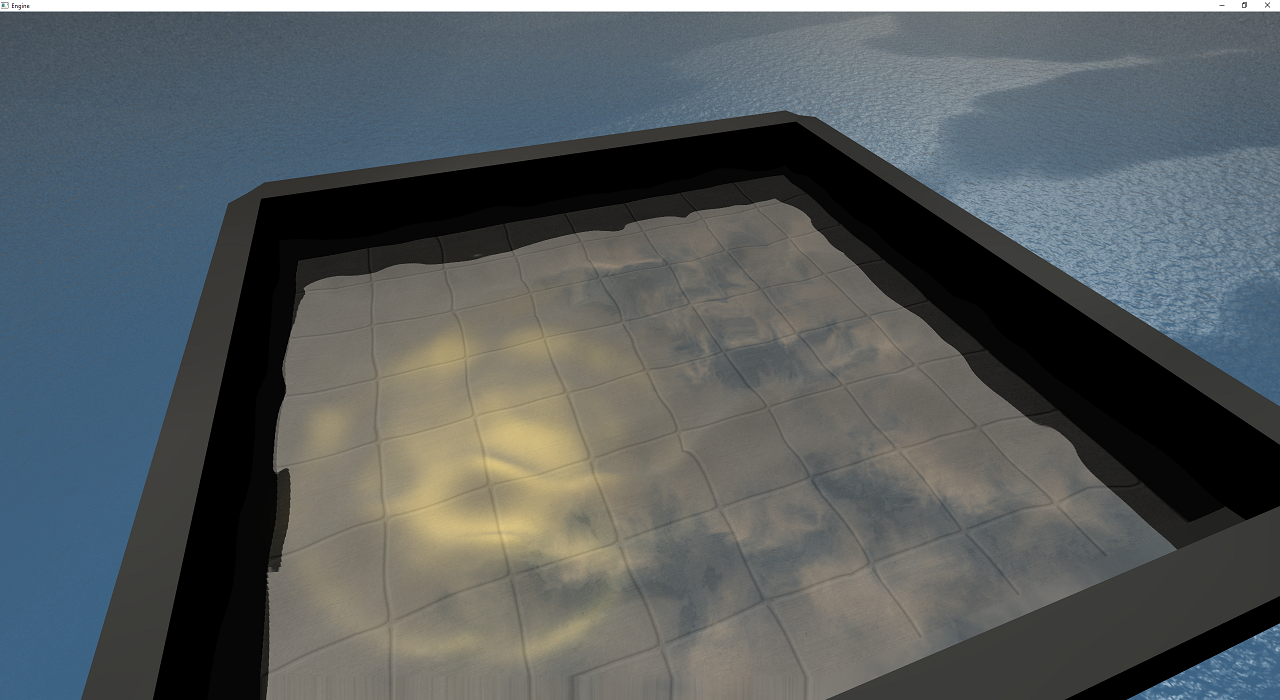
\includegraphics[width=0.9\textwidth]{./PhotoRapport/EffetFinal.png}
	\caption{Effet final}
	\label{EffetFinal}
\end{figure}
\begin{figure}
	\centering
	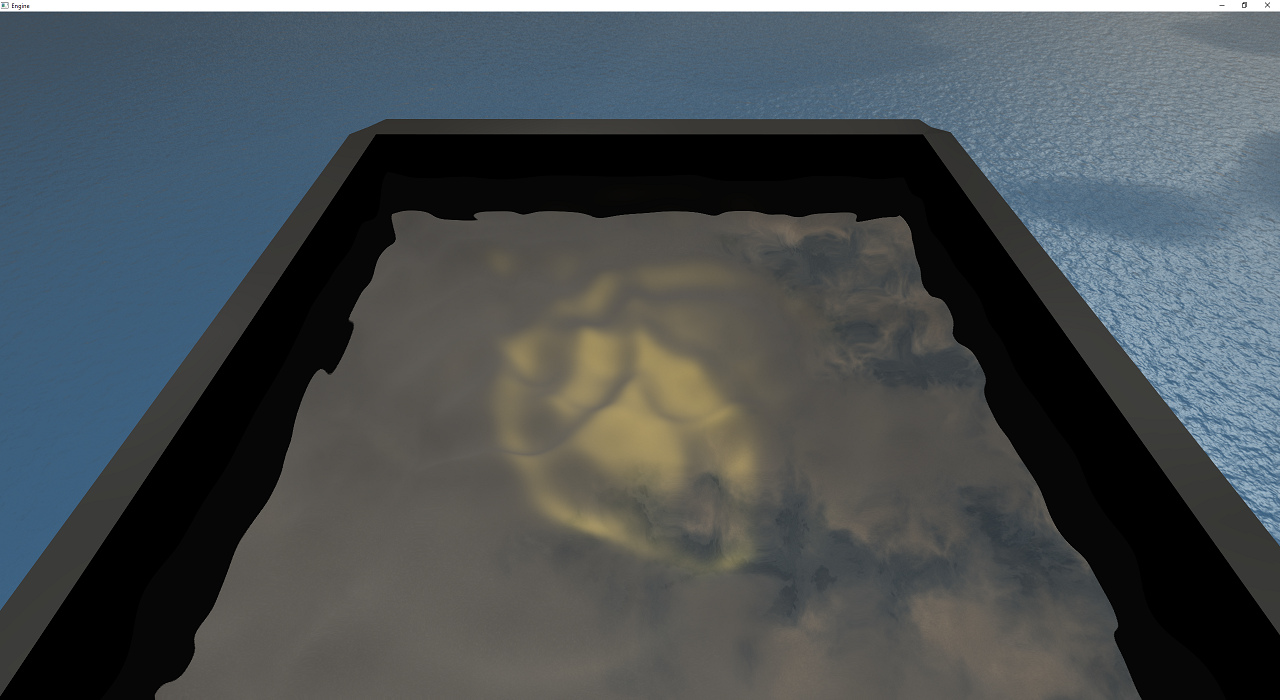
\includegraphics[width=0.9\textwidth]{./PhotoRapport/Reflection.png}
	\caption{Reflection}
	\label{Reflection}
\end{figure}
\begin{figure}
	\centering
	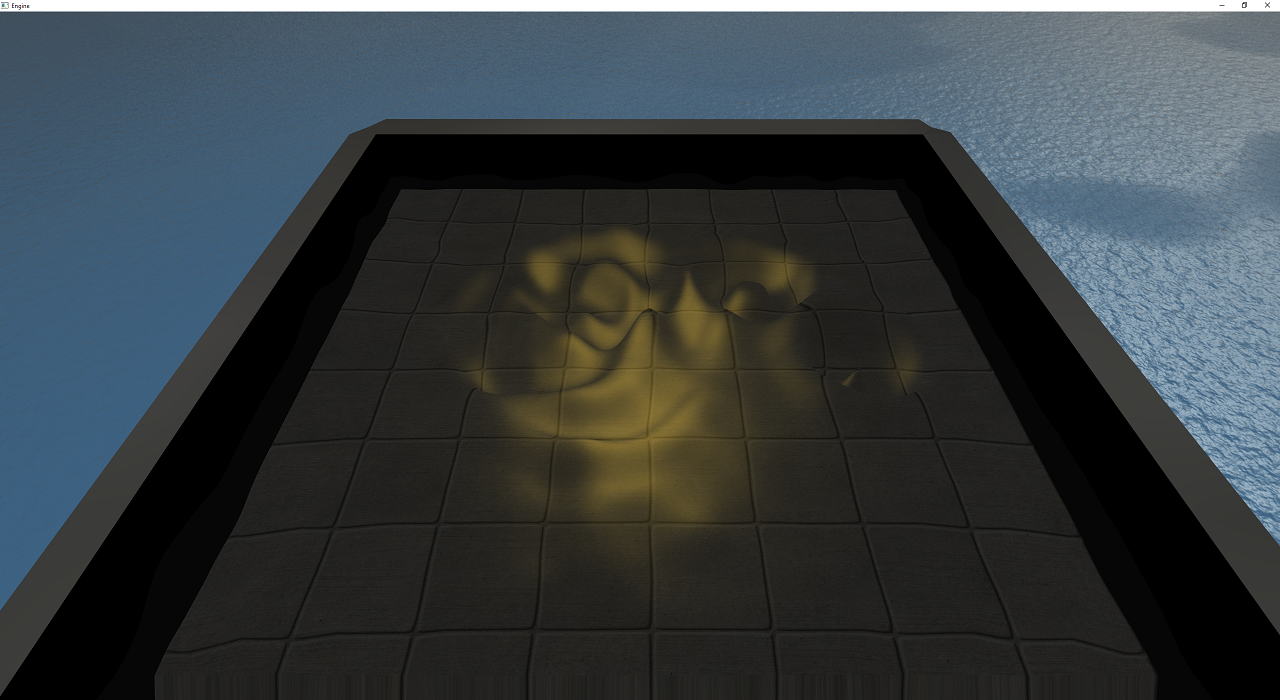
\includegraphics[width=0.9\textwidth]{./PhotoRapport/Refraction.png}
	\caption{Refraction}
	\label{Refractopm}
\end{figure}
\begin{figure}
	\centering
	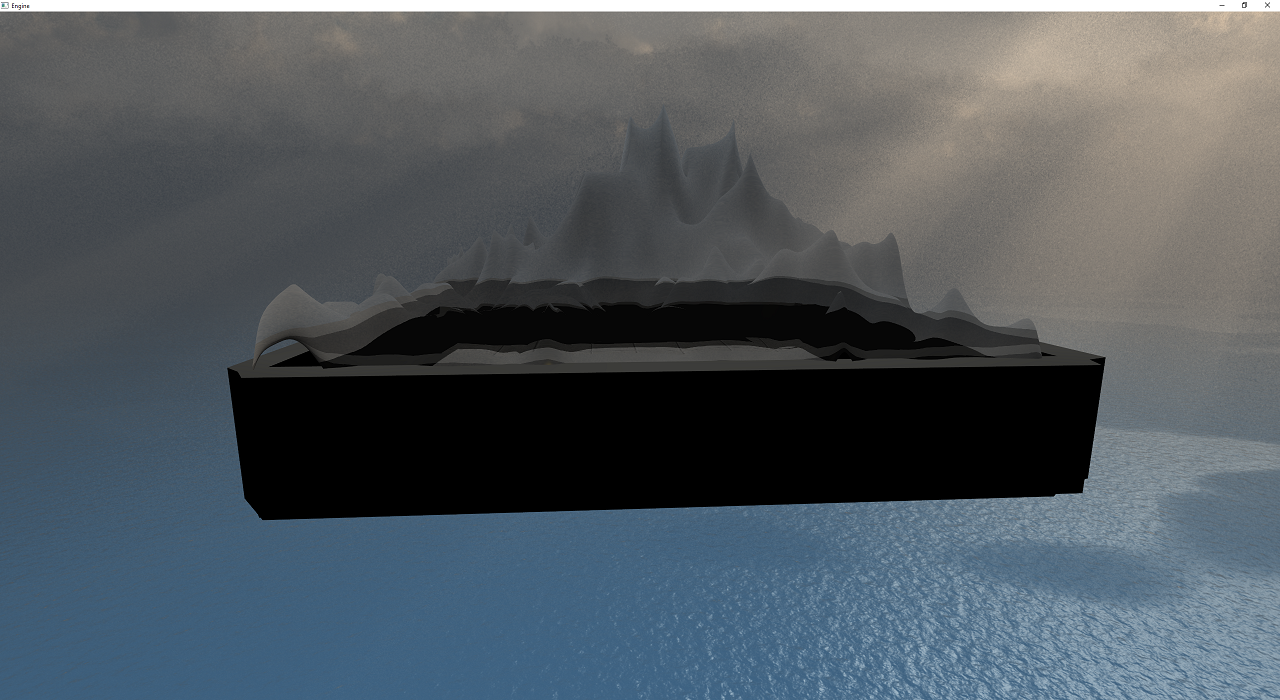
\includegraphics[width=0.9\textwidth]{./PhotoRapport/WaterConservation.png}
	\caption{Conservation d'eau}
	\label{WaterConservation}
\end{figure}
%----------------------------------------------------------------------------------------
\end{document}
